%% LaTeX Beamer presentation template (requires beamer package)
%% see http://latex-beamer.sourceforge.net/
%% idea contributed by H. Turgut Uyar
%% template based on a template by Till Tantau
%% this template is still evolving - it might differ in future releases!
\PassOptionsToPackage{footline=authorinstitutetitle}{beamerouterthememiniframes}
\documentclass{beamer}

\mode<presentation>
{
\useoutertheme[subsection=false]{miniframes}
\usetheme{Berlin}
\setbeamertemplate{navigation symbols}{} 
\setbeamercovered{dynamic}
\setbeamertemplate{footline}{}
}

\hypersetup{pdfstartview={FitH}}

\usepackage[brazilian]{babel}
\usepackage[utf8]{inputenc}
%\usepackage{mathptmx}% font definitions, try \usepackage{ae} instead of the following
%\usepackage[scaled=.90]{helvet}% three lines if you don't like this look
%\usepackage{courier}
\usepackage[T1]{fontenc}
\usepackage{lmodern}
\usepackage{url}


\title{Projeto Final: Proposta}
\subtitle{AUP2303 - Design de Tipos}

% - Use the \inst{?} command only if the authors have different
%   affiliation.
%\author{F.~Author\inst{1} \and S.~Another\inst{2}}
\author{Pedro Paulo Vezzá Campos - 7538743}

\date{\today}


% This is only inserted into the PDF information catalog. Can be left
% out.
\subject{Projeto Final Design de Tipos}



% If you have a file called "university-logo-filename.xxx", where xxx
% is a graphic format that can be processed by latex or pdflatex,
% resp., then you can add a logo as follows:

% \pgfdeclareimage[height=0.5cm]{university-logo}{university-logo-filename}
% \logo{\pgfuseimage{university-logo}}



% Delete this, if you do not want the table of contents to pop up at
% the beginning of each subsection:
\AtBeginSection[]
{
\begin{frame}<beamer>
\frametitle{Sumário}
\tableofcontents[currentsection,currentsubsection]
\end{frame}
}

% If you wish to uncover everything in a step-wise fashion, uncomment
% the following command:

%\beamerdefaultoverlayspecification{<+->}

\begin{document}

\begin{frame}
\titlepage
\end{frame}

\begin{frame}
\frametitle{Sumário}
\tableofcontents
% You might wish to add the option [pausesections]
\end{frame}


\section{Ideia}
\subsection{}

\begin{frame}
\frametitle{Lego Mindstorms	Education}
%\usepackage{graphics} is needed for \includegraphics
\begin{figure}[htp]
\begin{center}
  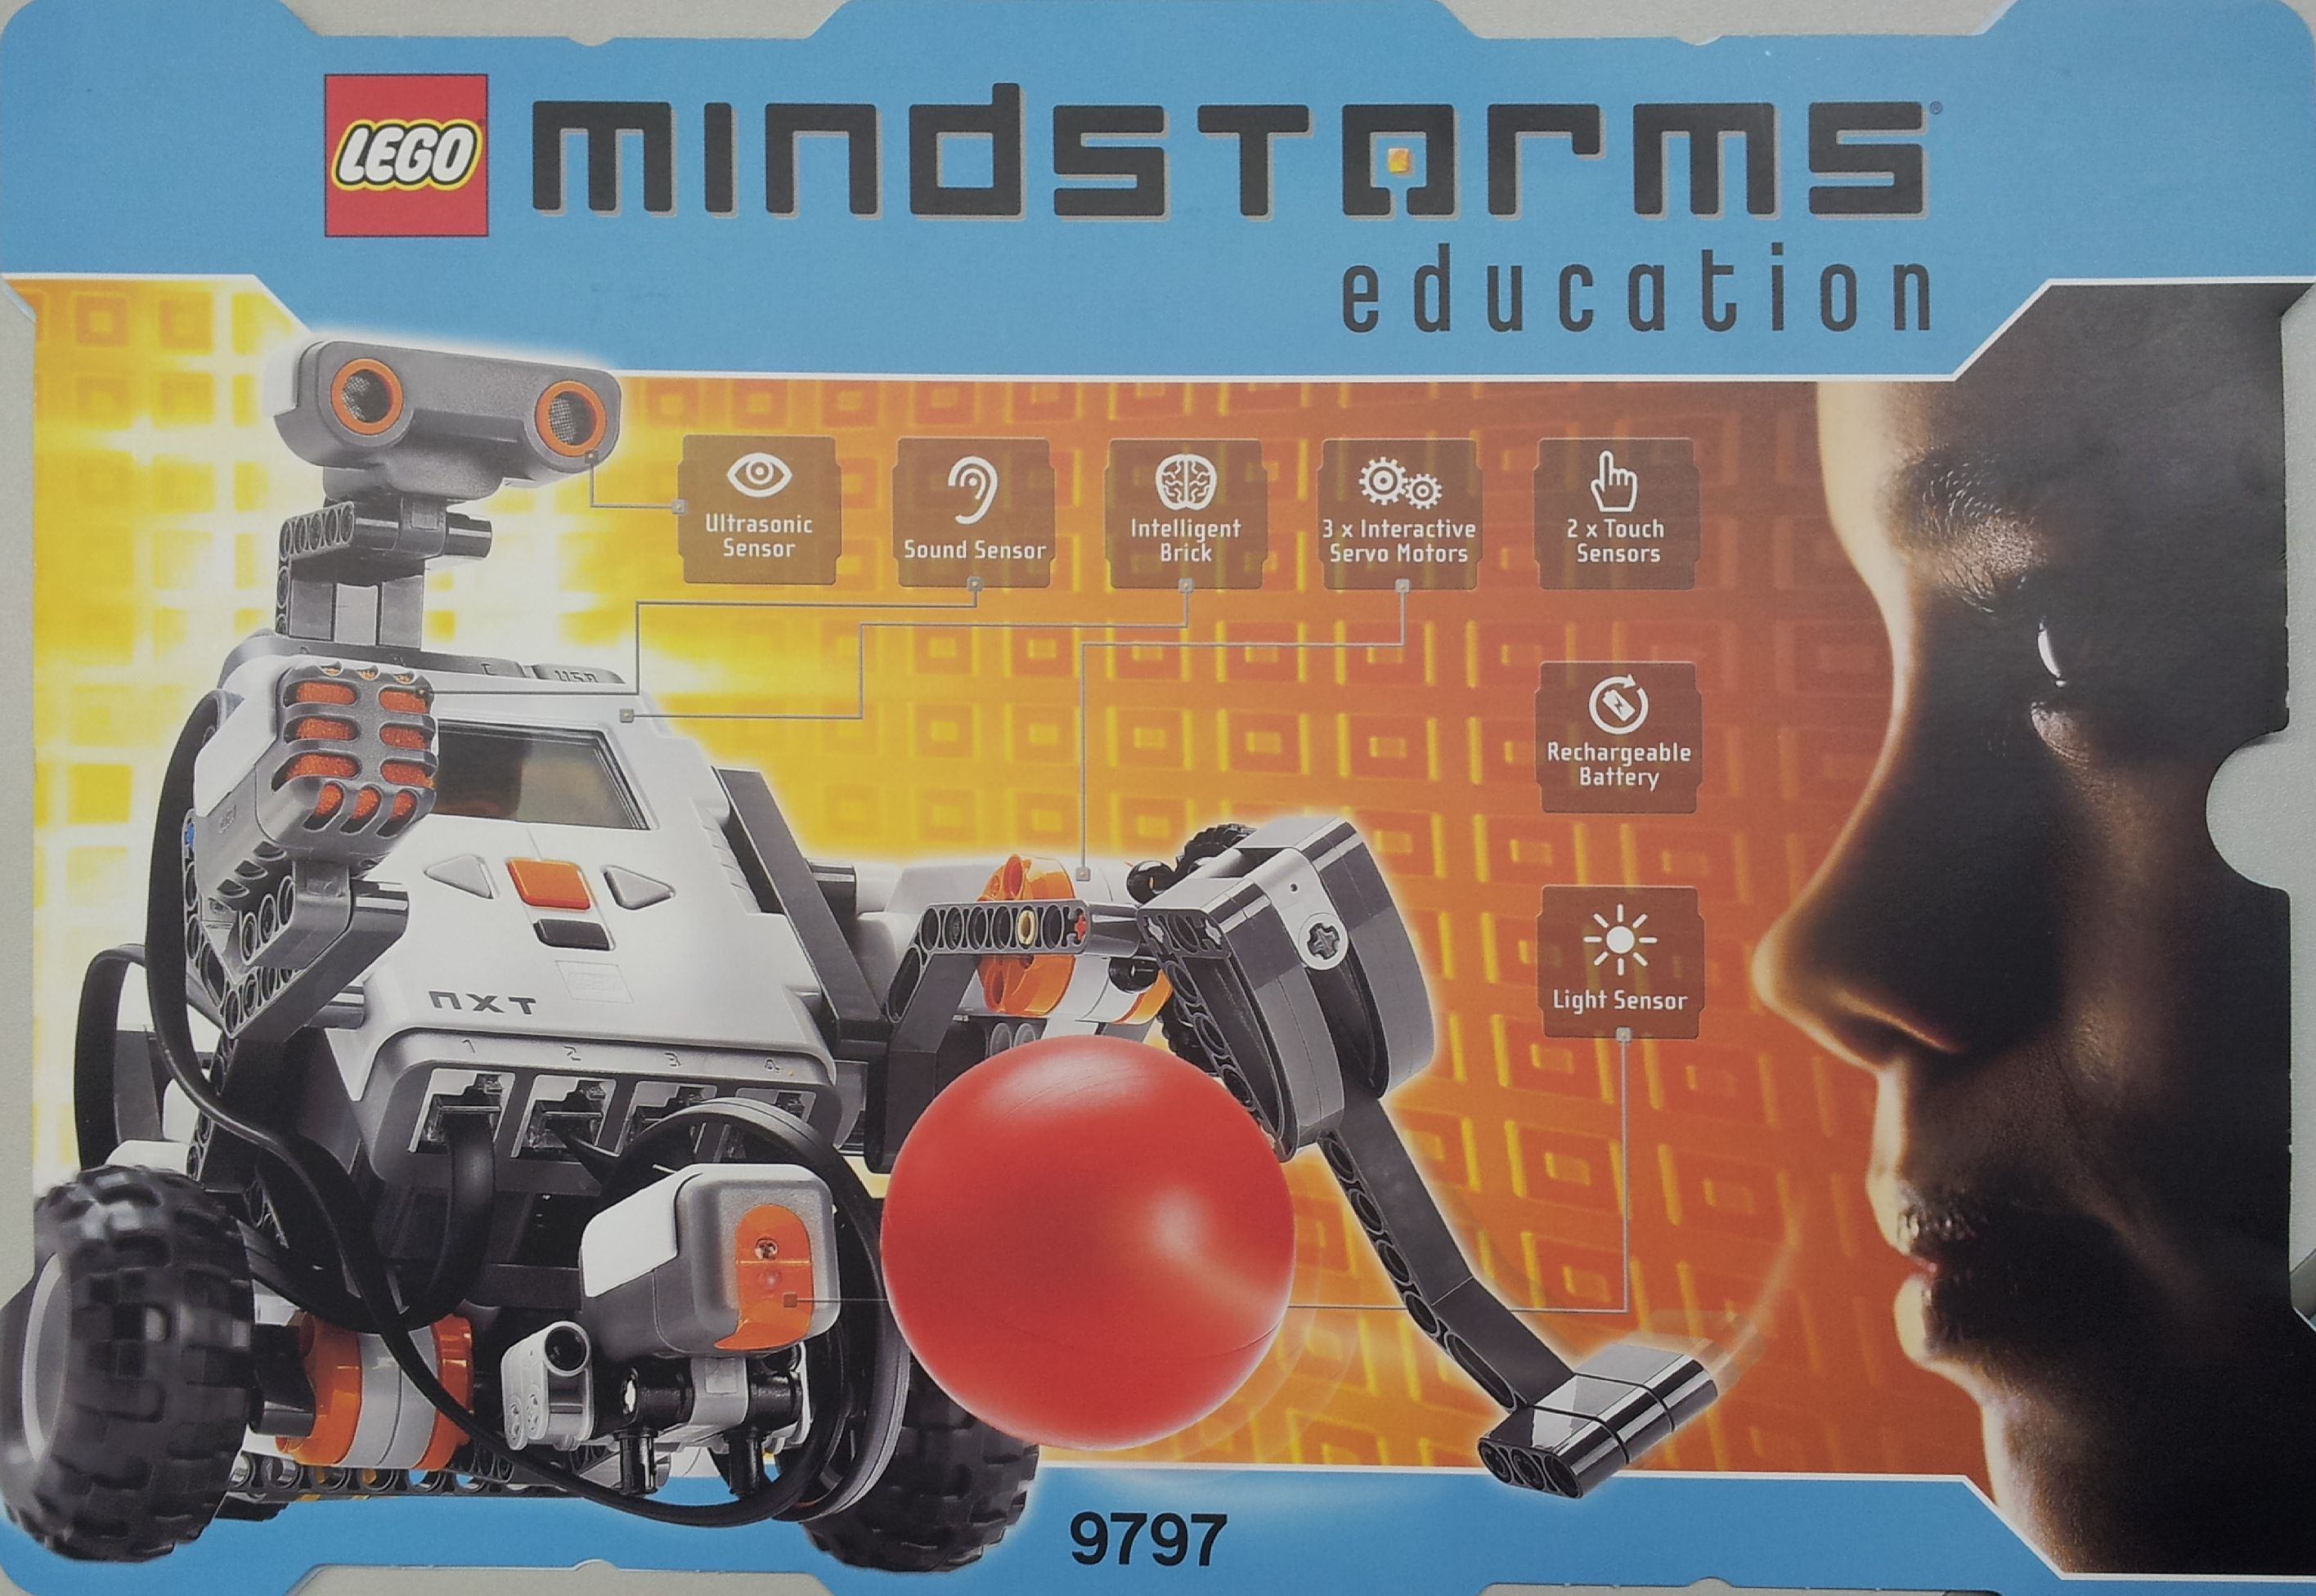
\includegraphics[width=\linewidth]{imagens/pecas-003.jpg}
%  \caption[dlink]{DI-604: 100 Mbps, \$60}
%  \label{dlink}
\end{center}
\end{figure}
\end{frame}

\begin{frame}
\frametitle{Lego Mindstorms	Education}
%\usepackage{graphics} is needed for \includegraphics
\begin{figure}[htp]
\begin{center}
  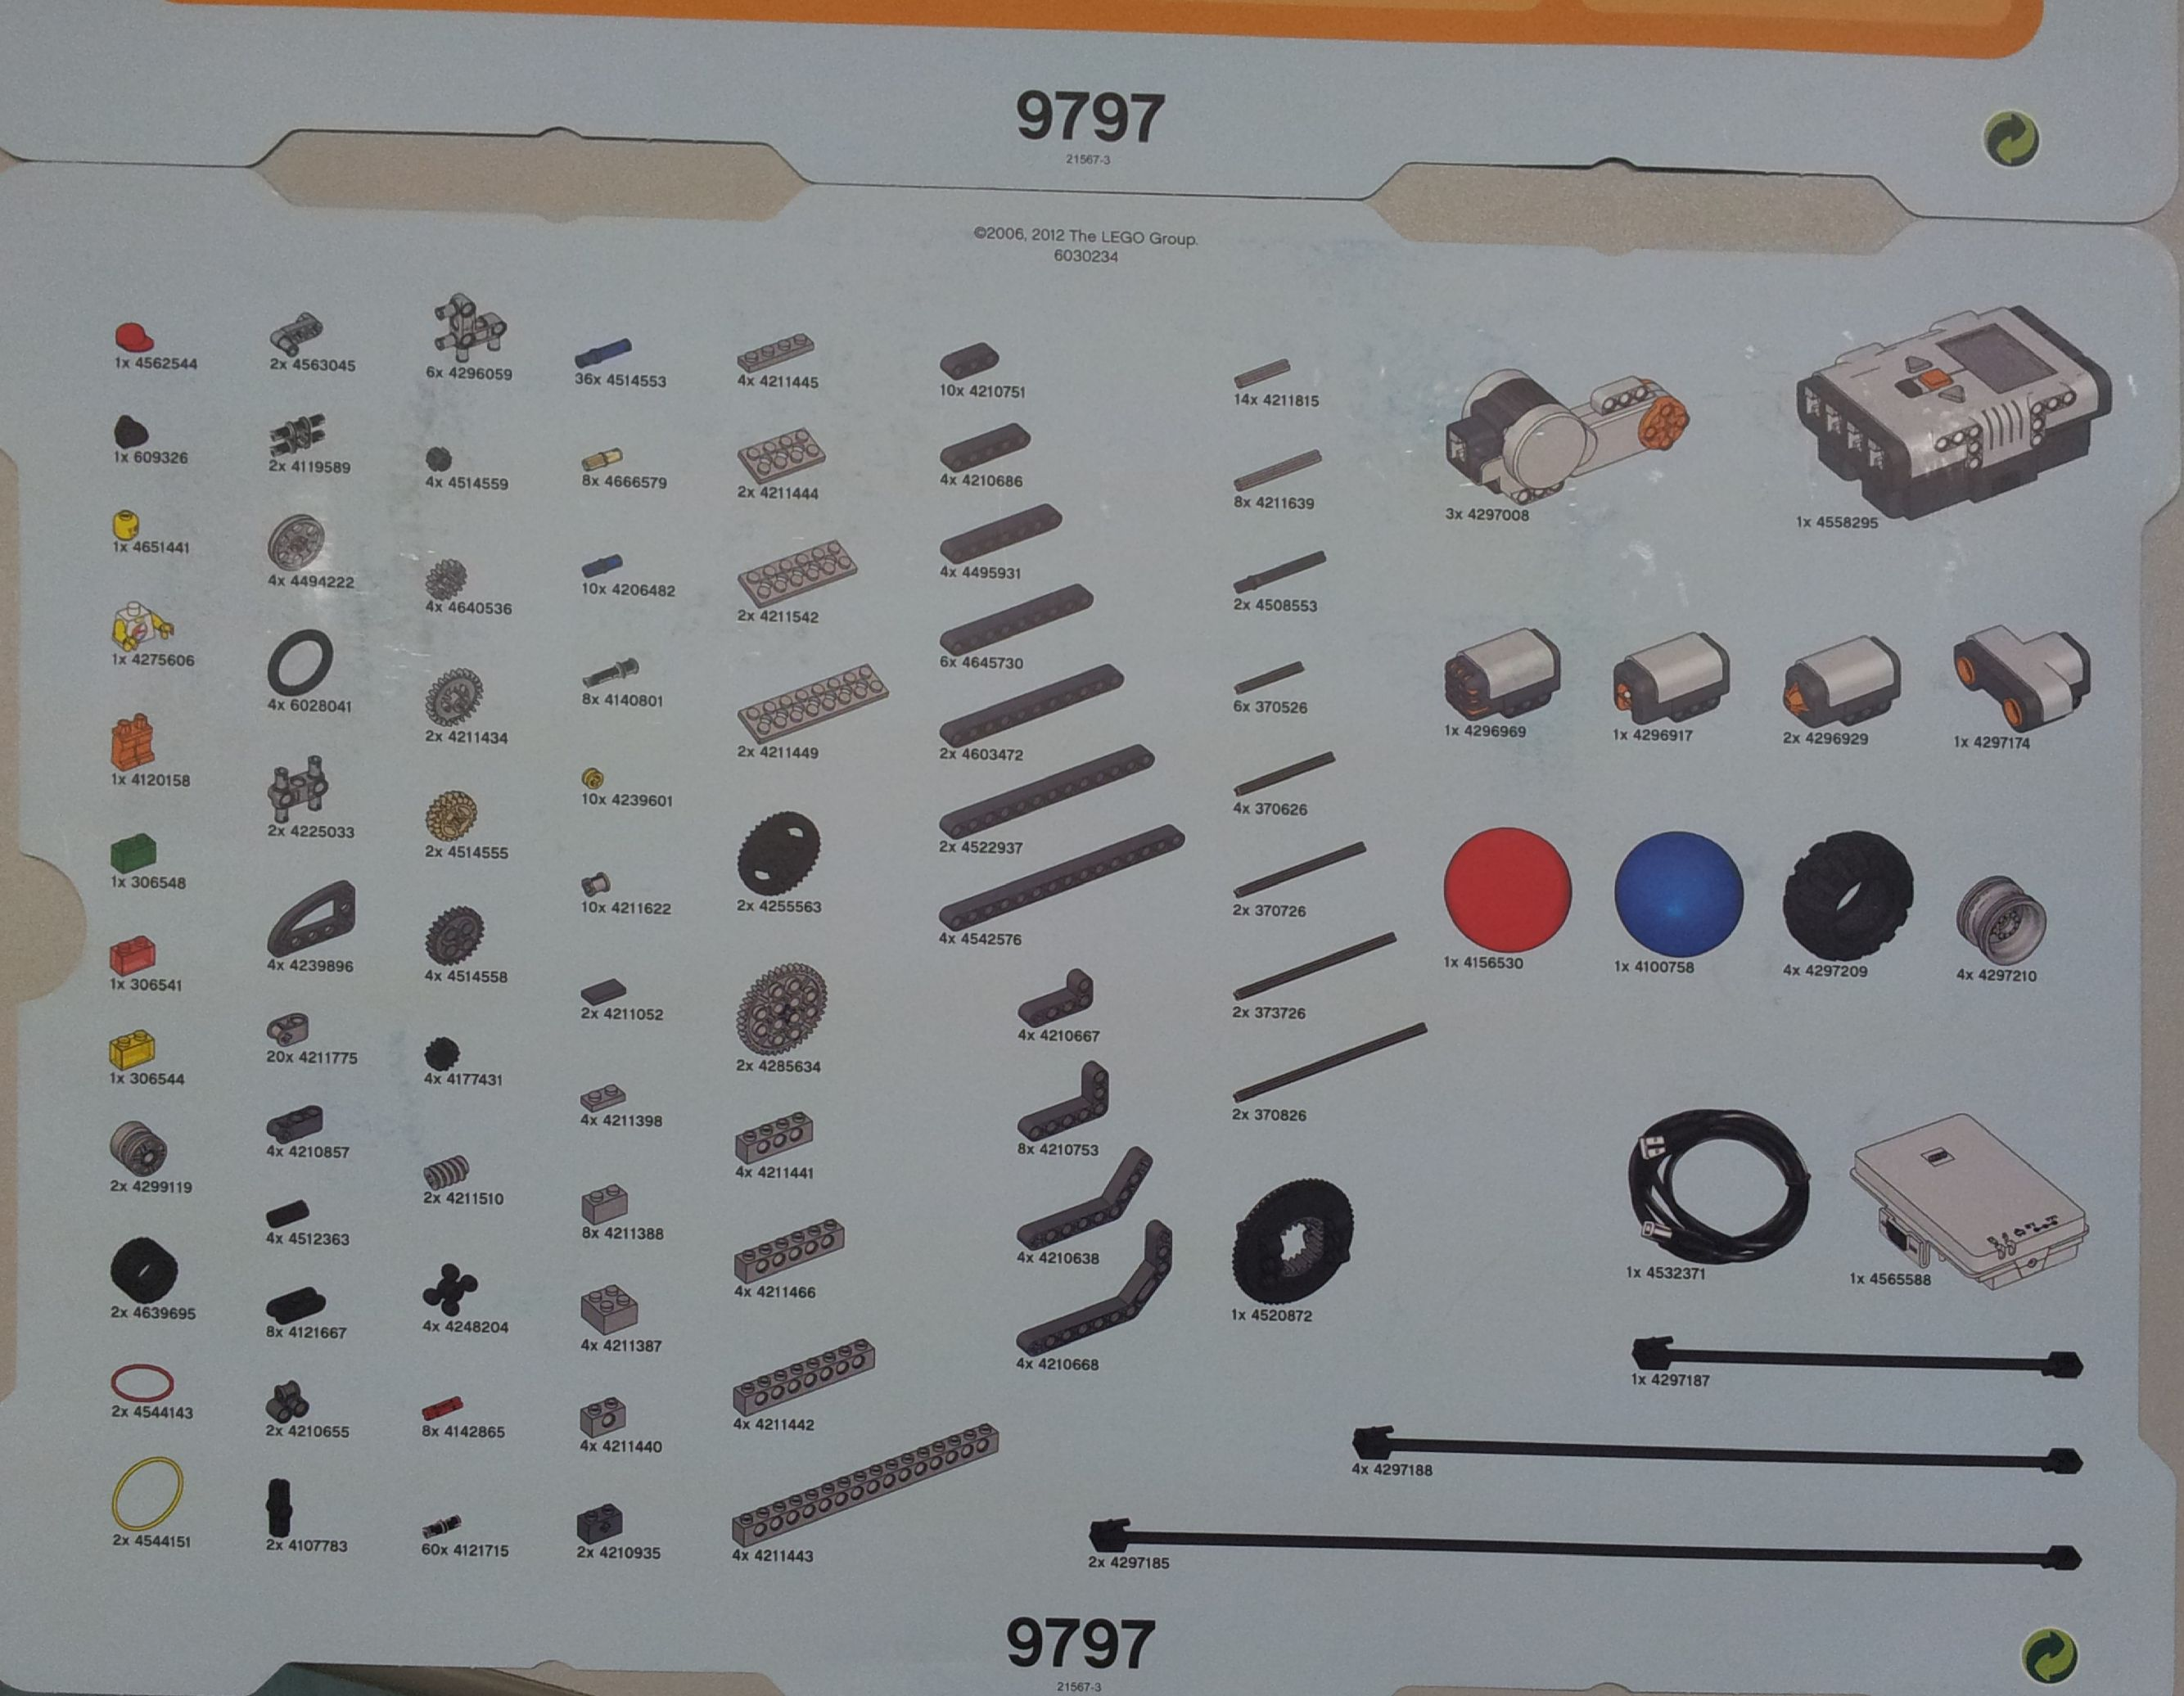
\includegraphics[width=90mm]{imagens/pecas-000.jpg}
%  \caption[dlink]{DI-604: 100 Mbps, \$60}
%  \label{dlink}
\end{center}
\end{figure}
\end{frame}

\begin{frame}
\frametitle{Lego Mindstorms	Education}
%\usepackage{graphics} is needed for \includegraphics
\begin{figure}[htp]
\begin{center}
  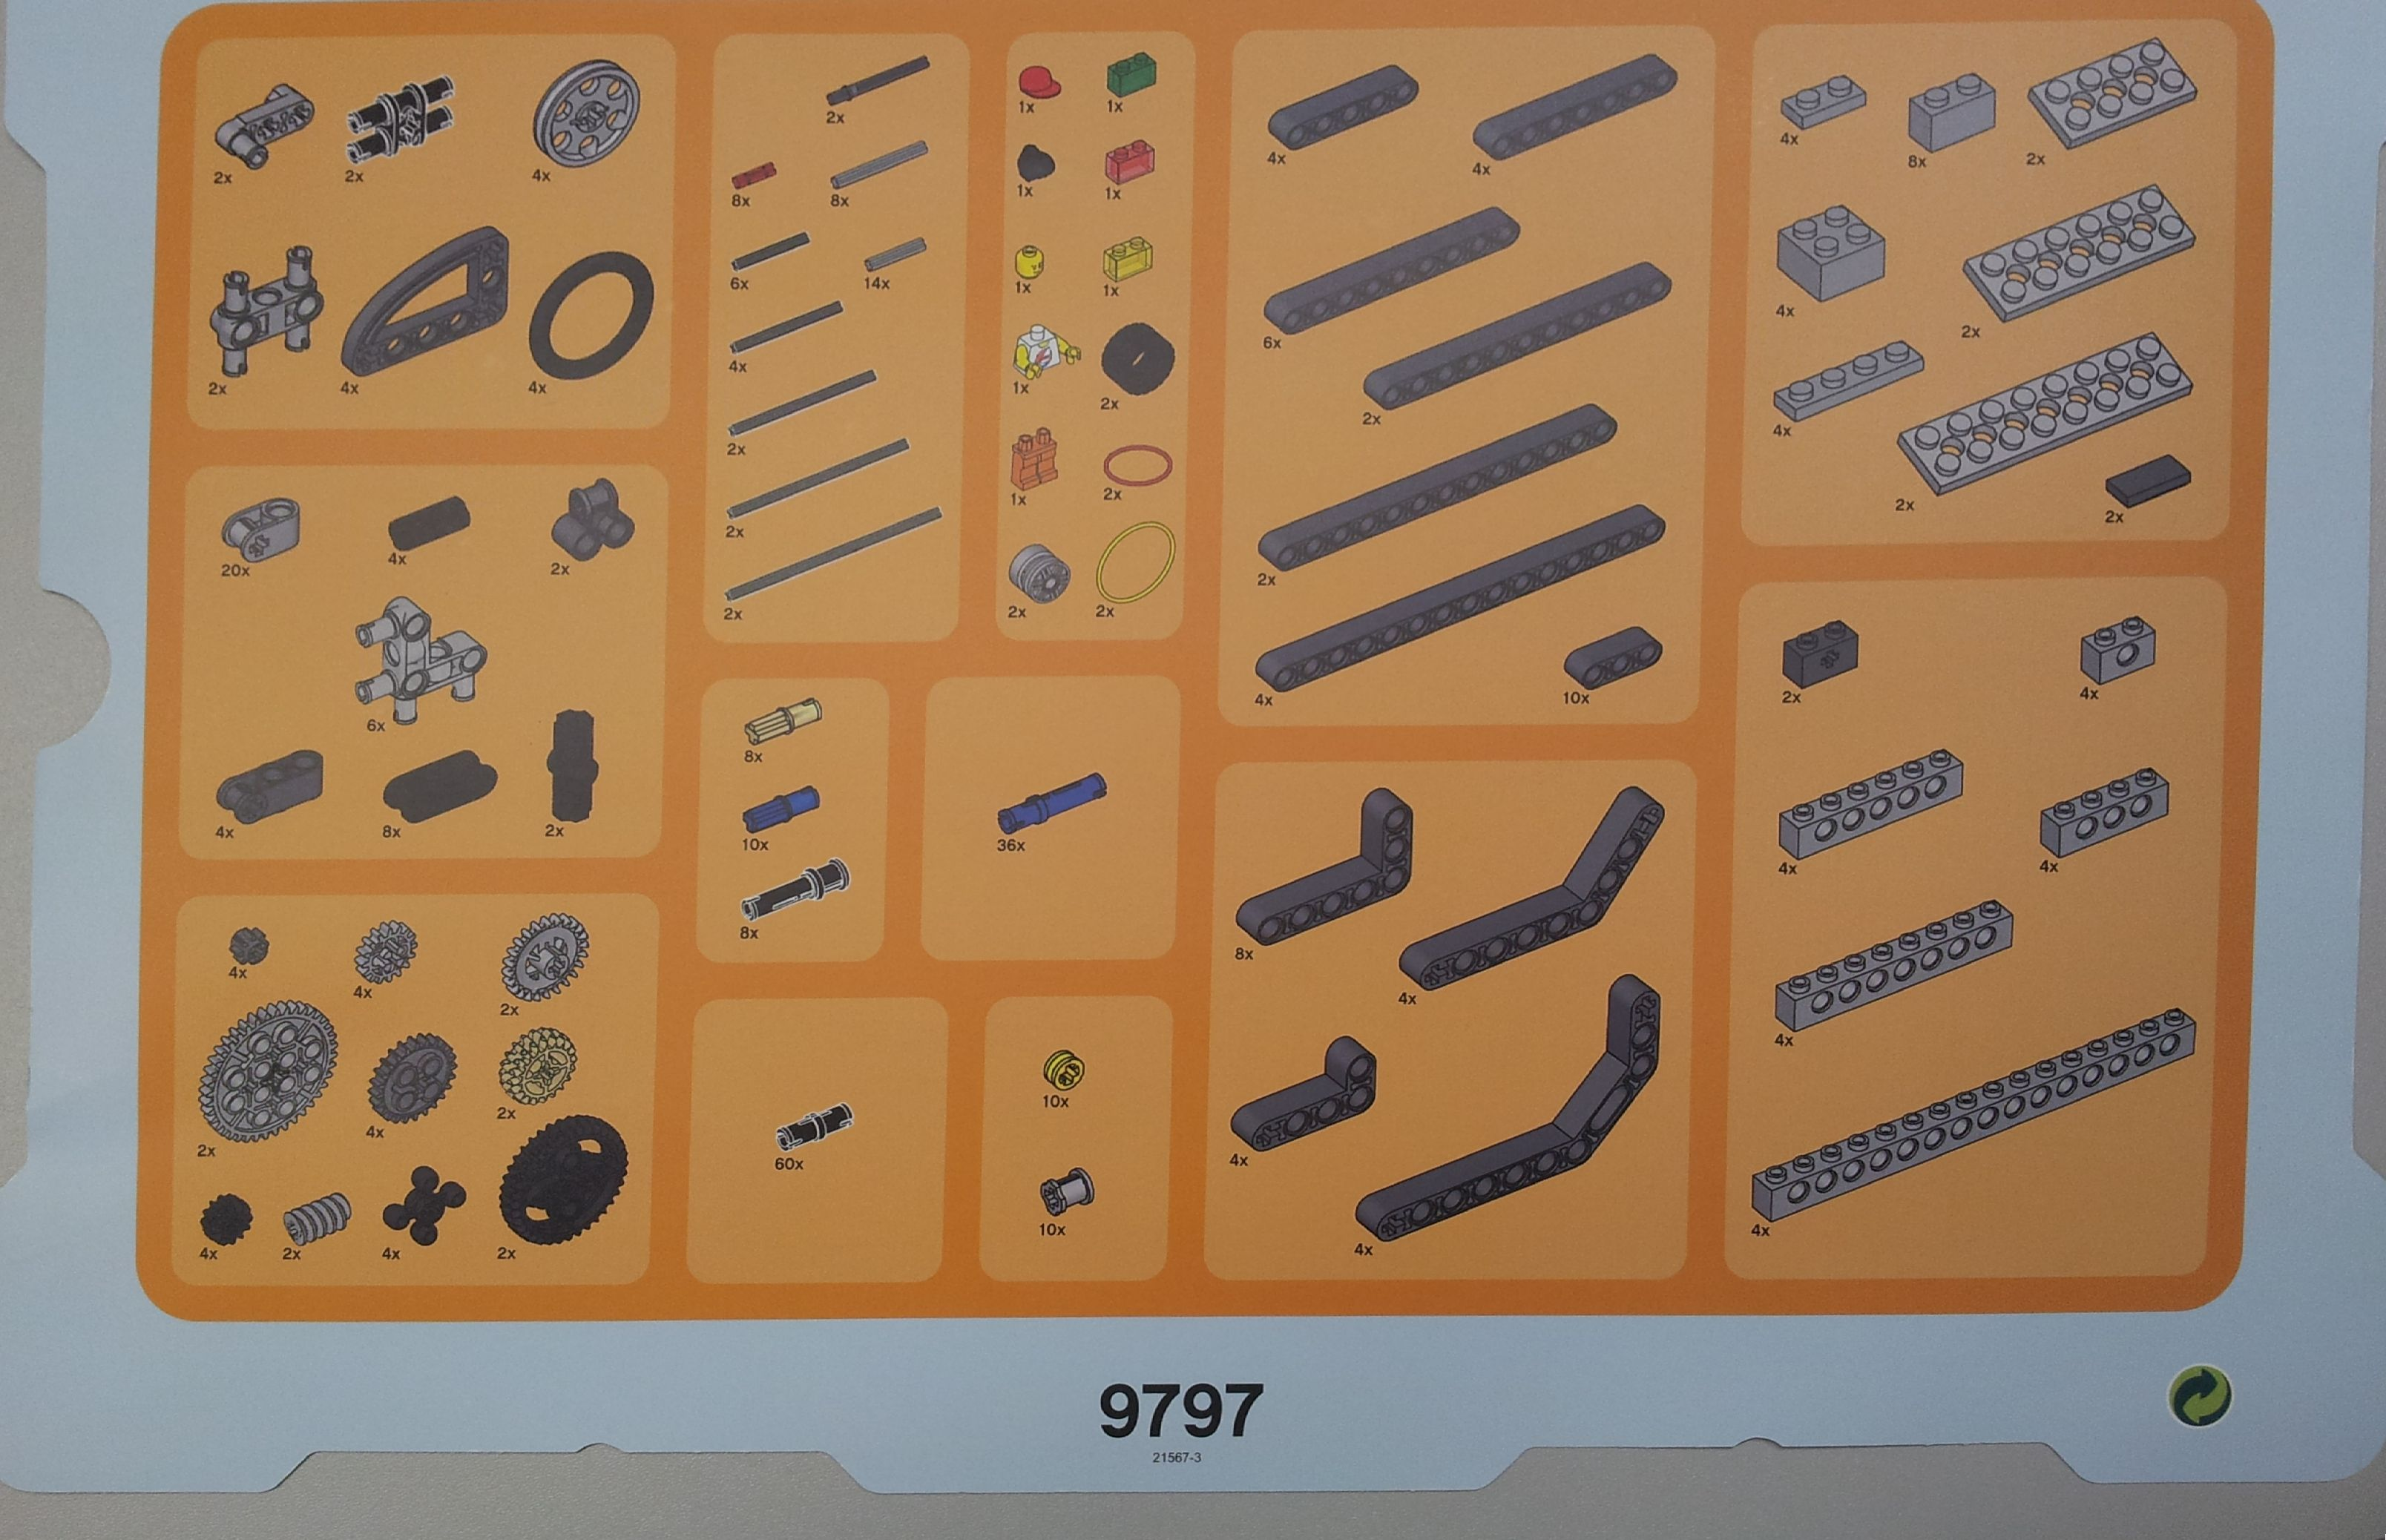
\includegraphics[width=\linewidth]{imagens/pecas-001.jpg}
%  \caption[dlink]{DI-604: 100 Mbps, \$60}
%  \label{dlink}
\end{center}
\end{figure}
\end{frame}

\begin{frame}
\frametitle{Lego Mindstorms	Education}
%\usepackage{graphics} is needed for \includegraphics
\begin{figure}[htp]
\begin{center}
  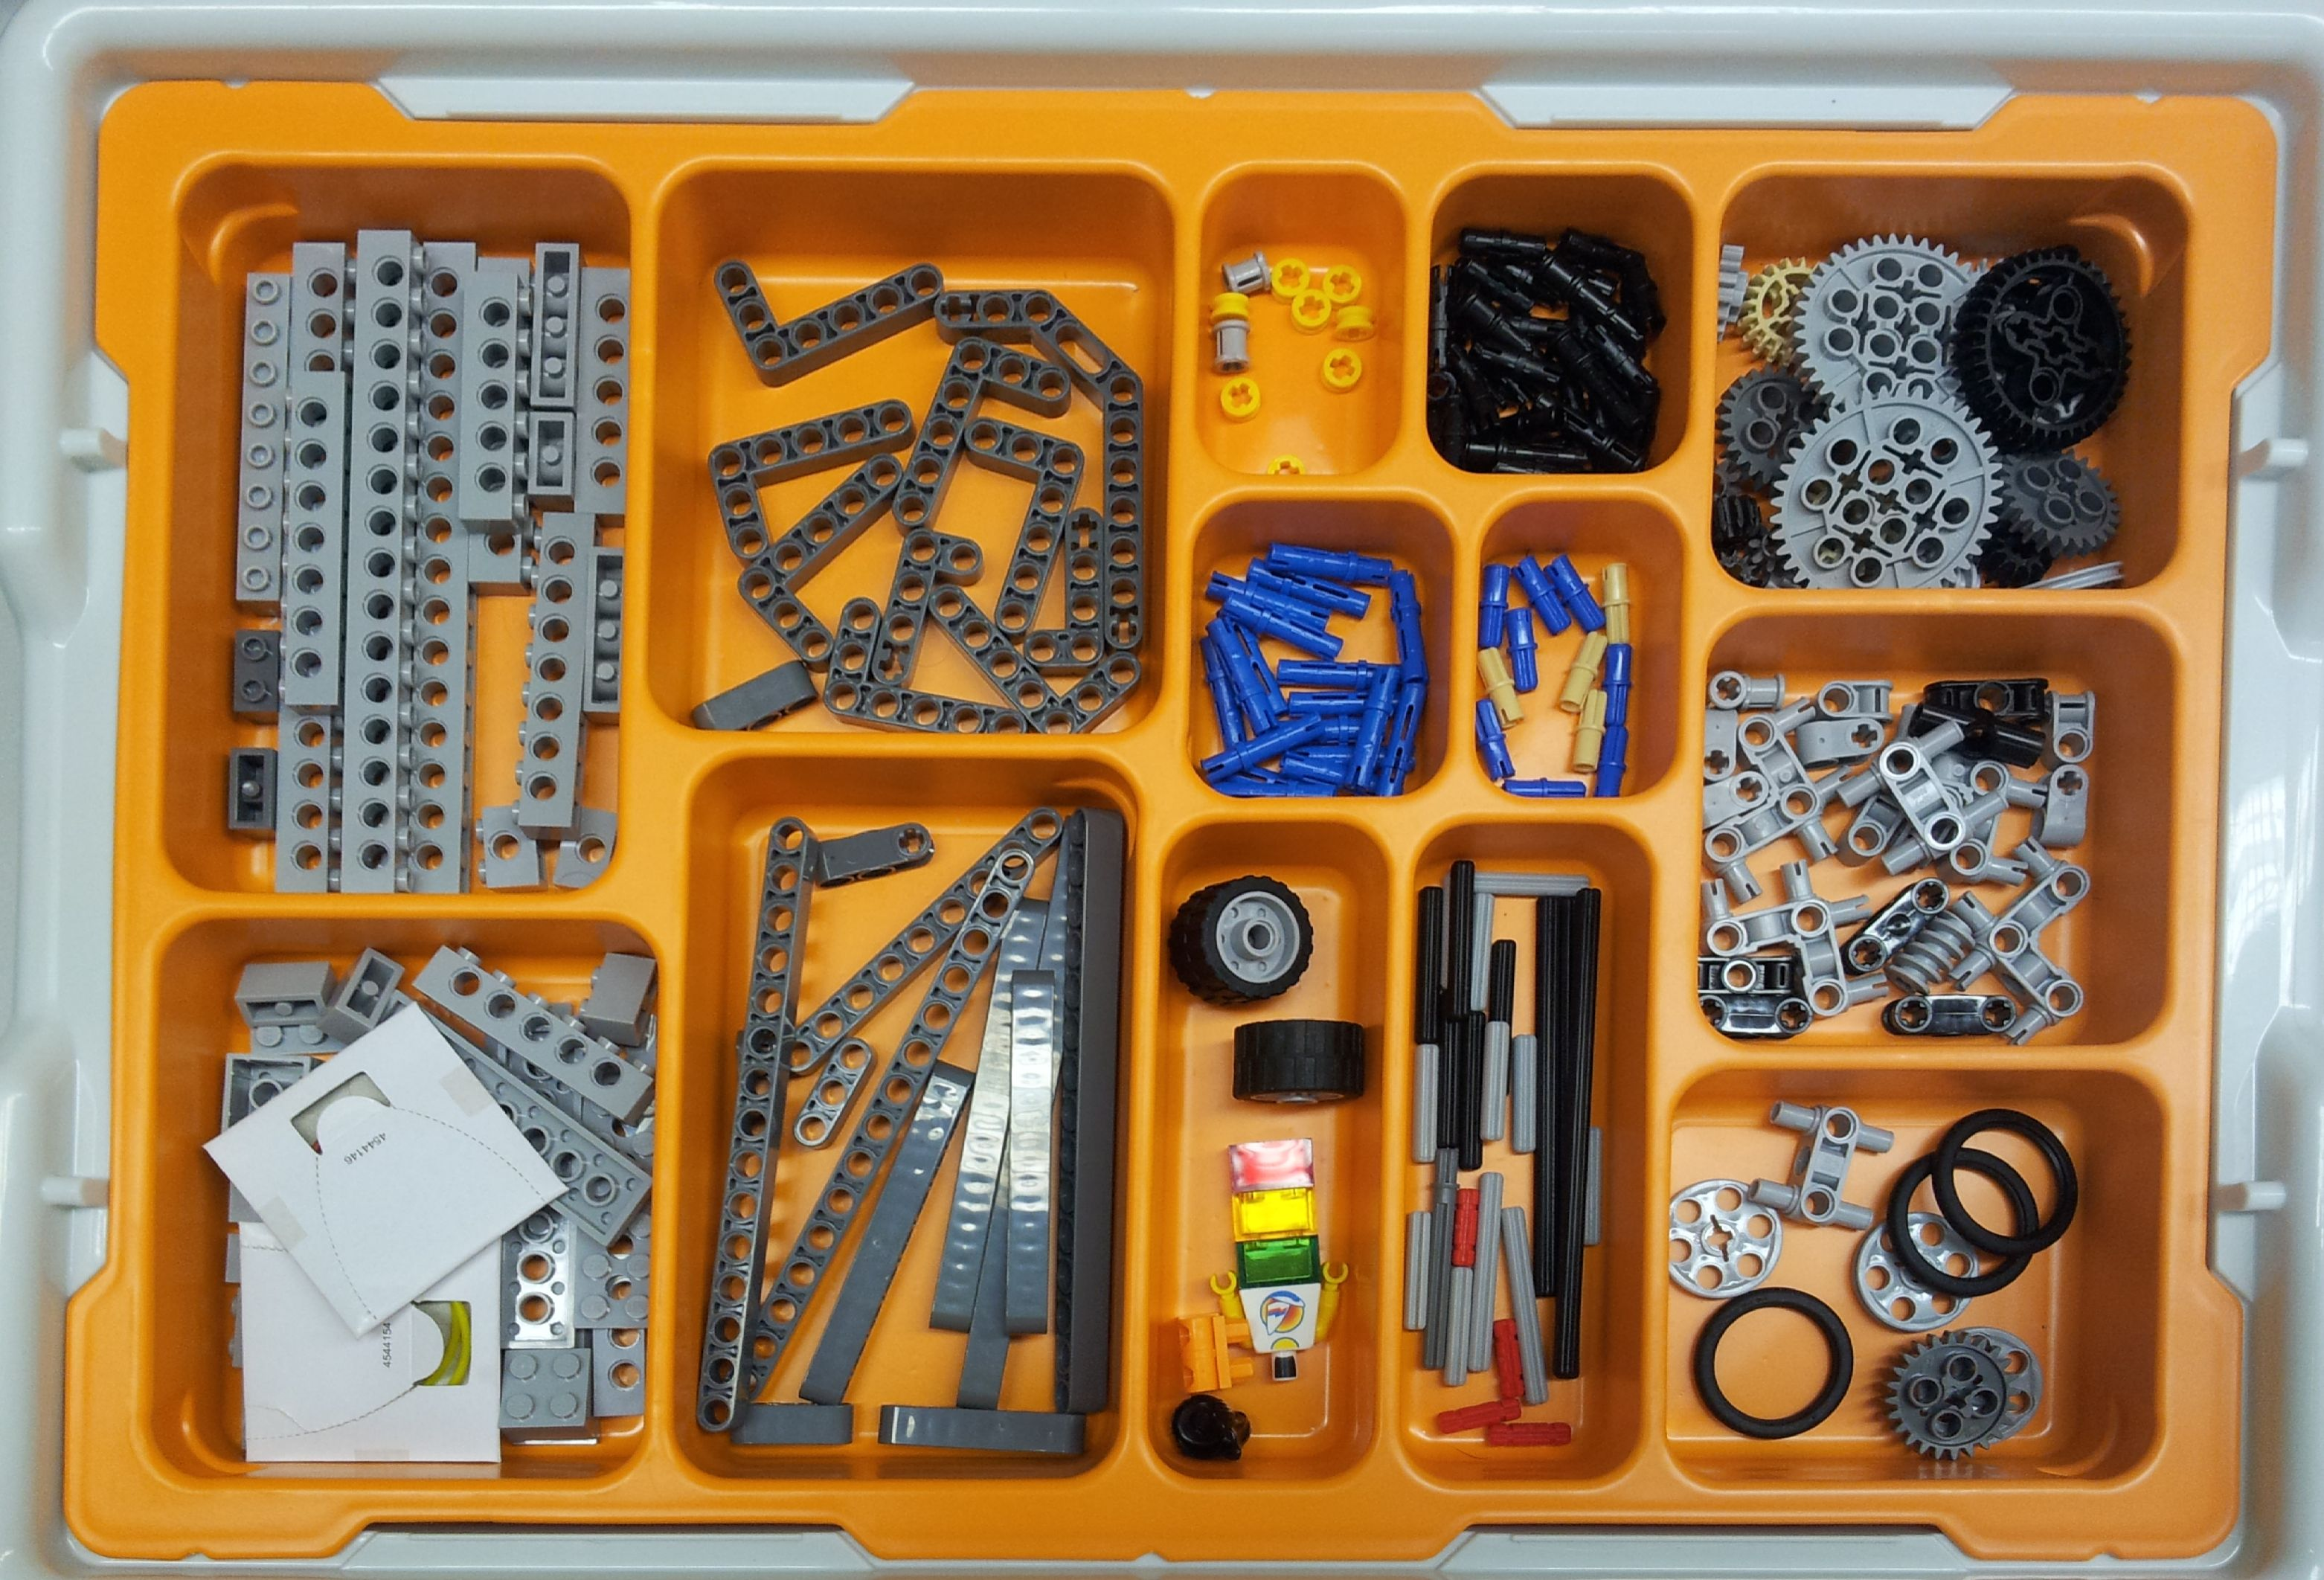
\includegraphics[width=\linewidth]{imagens/pecas-002.jpg}
%  \caption[dlink]{DI-604: 100 Mbps, \$60}
%  \label{dlink}
\end{center}
\end{figure}
\end{frame}

\section{Proposta}
\subsection{}

\begin{frame}
\frametitle{Vetorizar algumas peças (todas?)}
%\usepackage{graphics} is needed for \includegraphics
\begin{figure}[htp]
\begin{center}
  
\includegraphics[width=\linewidth]{imagens/pecas-004.jpg}
%  \caption[dlink]{DI-604: 100 Mbps, \$60}
%  \label{dlink}
\end{center}
\end{figure}
\end{frame}

\begin{frame}
\frametitle{Protótipo: Caracteres chave com design modular}
%\usepackage{graphics} is needed for \includegraphics
\begin{figure}[htp]
\begin{center}
  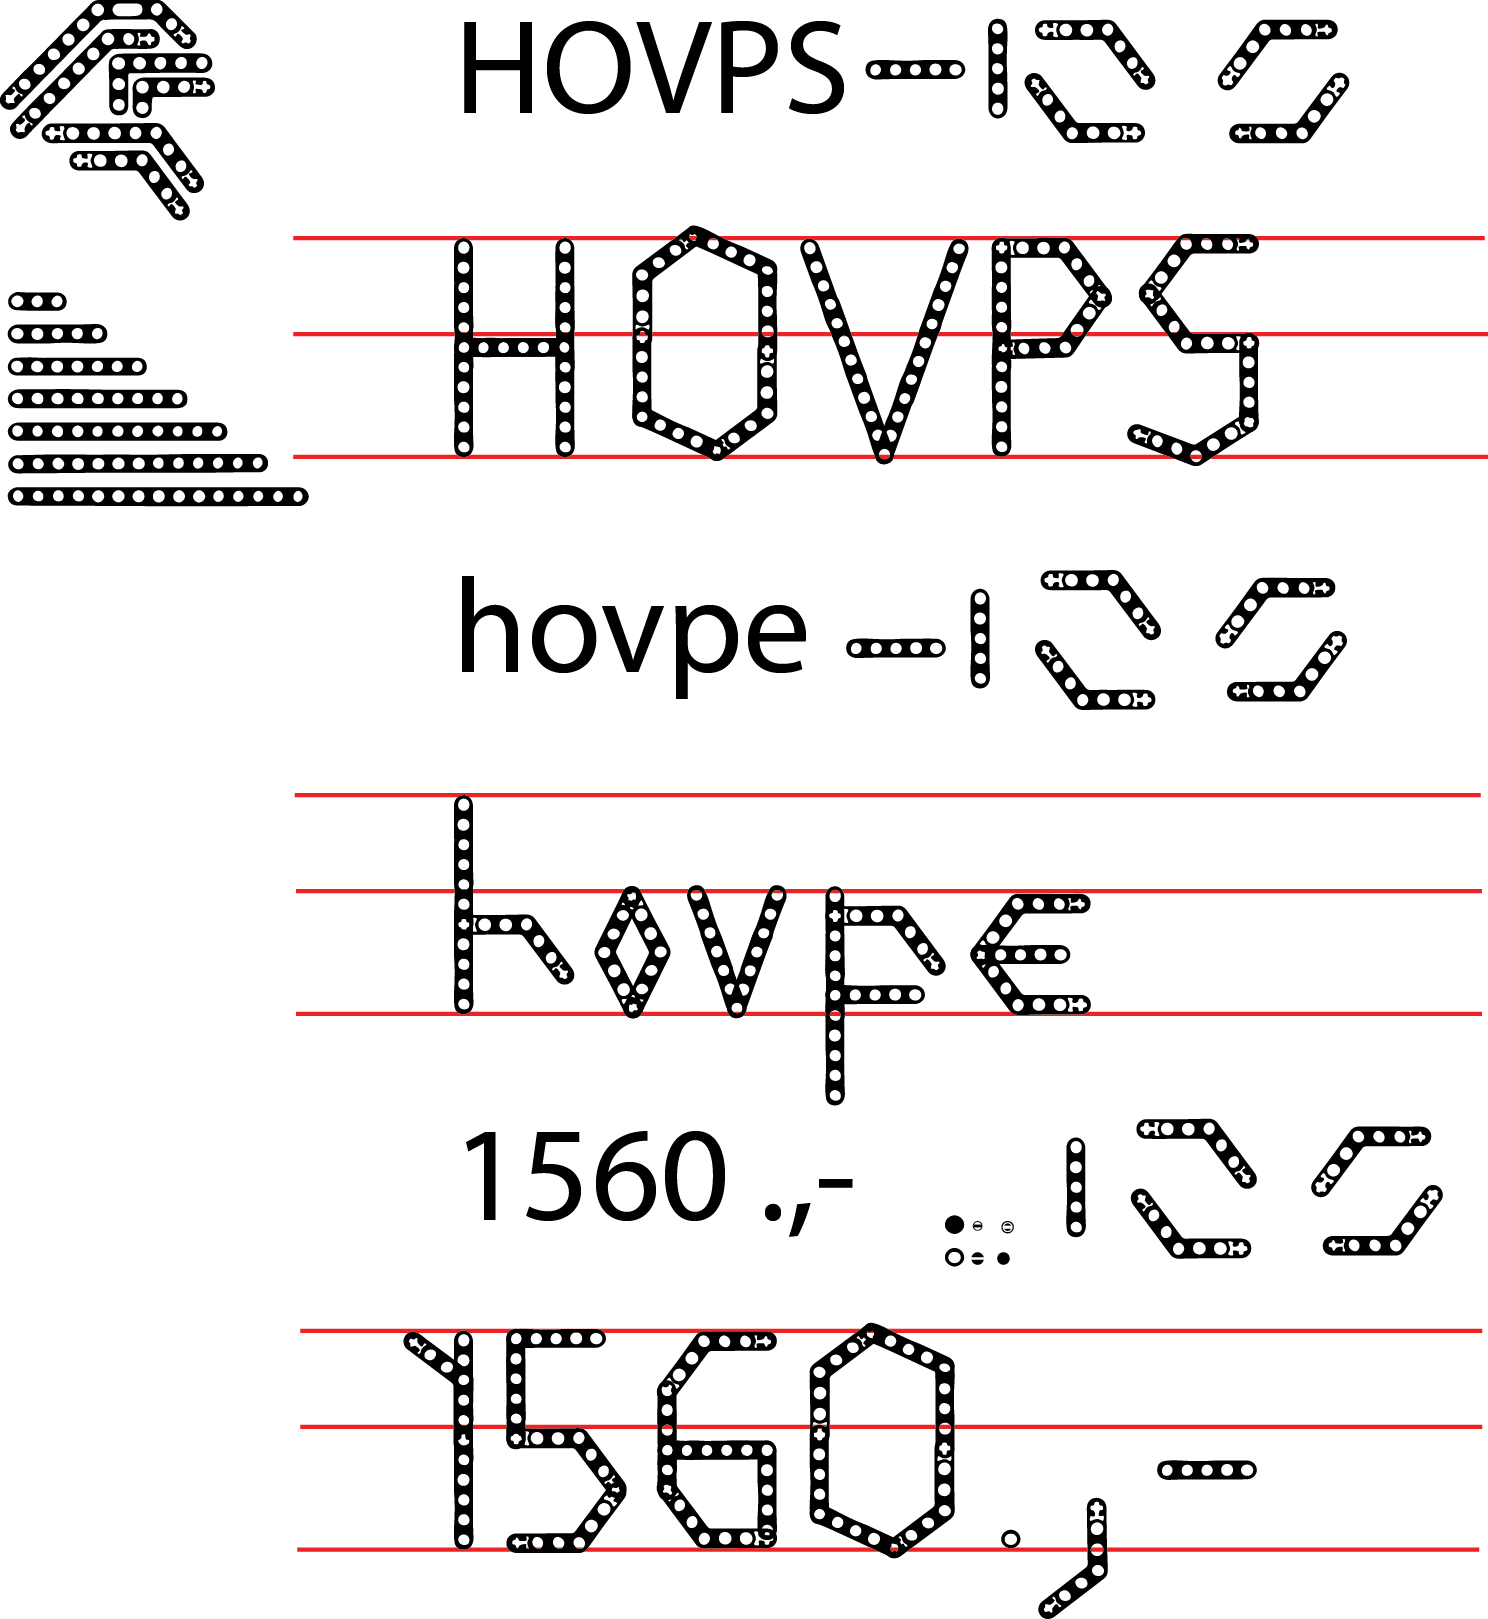
\includegraphics[width=60mm]{imagens/Lego.png}
%  \caption[dlink]{DI-604: 100 Mbps, \$60}
%  \label{dlink}
\end{center}
\end{figure}
\end{frame}

\begin{frame}
\frametitle{Protótipo: Caracteres chave com design modular}
%\usepackage{graphics} is needed for \includegraphics
\begin{figure}[htp]
\begin{center}
  
\includegraphics[width=\linewidth]{imagens/Lego1Linha.png}
%  \caption[dlink]{DI-604: 100 Mbps, \$60}
%  \label{dlink}
\end{center}
\end{figure}
\end{frame}

\end{document}

